% ====================================================
\section{Numerical results}\label{sec:Num_Result}
% ====================================================
We present numerical experiments to demonstrate the efficacy of the proposed iterative integer-valued sample size allocation scheme. The method is compared against three benchmarks: (i) the standard real-valued MFMC allocation, (ii) direct flooring of the real-valued solution, and (iii) the modified rounding approach of \cite{GrGuJuWa:2023}. Performance is evaluated through both allocation efficiency and the resulting estimator variance under fixed computational budgets.

\subsection{First example}
Table~\ref{Tab:Eg1_Parameters} summarizes the model parameters derived from a plasma physics application \cite{ElLiSa:2023,ElLiSa:2025}, featuring five fidelity levels with strongly correlated models ($\rho_{1,k} > 0.98$) and rapidly decreasing computational costs across the hierarchy.


Table~\ref{tab:MFMC_integer_comparison_Eg1} presents detailed allocation comparisons for two budget scenarios. For $p=200$, the real-valued allocation achieves the theoretical optimum with variance $f=2.1645\times10^{-4}$. Direct flooring reduces the actual cost to approximately 169.86 (15\% budget underutilization) while increasing variance by 18\%. In contrast, the iterative scheme fully utilizes the budget ($p=200$) and maintains variance within 11\% of the continuous optimum.


The constrained budget case ($p=73.03$) reveals more dramatic differences. Direct flooring produces a degenerate estimator (infinite variance) by assigning zero samples to the highest-cost model. The modified approach restores feasibility but yields substantially higher variance ($f=2.4834\times10^{-2}$). The iterative method achieves a 5\% variance reduction relative to the modified approach while maintaining full budget utilization, demonstrating its ability to balance constraint satisfaction with statistical efficiency.

%
\begin{table}[ht]
\centering
\scalebox{1}{
\begin{tabular}{|c|c|c|c|c|c|c|}
\hline
Model index &1 &2 &3 &4 &5 \\
\hline
Correlation coeff $\rho_{1,k}$ &1     &9.9977e-01   &9.9925e-01  &9.9728e-01   &9.8390e-01\\
% \hline
% Standard deviation $\sigma_k$ &1.0840e-02    &1.0838e-02   &1.1001e-02  &1.1549e-02   &9.5720e-03\\
\hline
Cost &73&7.0318e-03 &1.4018e-03 &5.0613e-04 &2.6803e-04\\
\hline
\end{tabular}
}
\caption{Model parameters for the plasma physics example.}
\label{Tab:Eg1_Parameters}
\end{table}
%


\begin{table}[ht]
\centering
\scalebox{0.73}{
\begin{tabular}{|c|p{4.8cm}|c|c|p{4.8cm}|c|c|}
\hline
\multirow{2}{*}{Method} 
& \multicolumn{3}{c|}{$p = 73.03$} 
& \multicolumn{3}{c|}{$p = 200$} \\
\cline{2-7}
& Sample size & Total cost & $f$ 
& Sample size & Total cost & $f$ \\
\hline
Real-valued 
& [8.8106e-01, 1.3495e+02, 5.8795e+02, 2.5402e+03, 2.1095e+04] 
& 7.3029e+01 & 5.9275e-04 
& [2.4129e+00, 3.6959e+02, 1.6102e+03, 6.9567e+03, 5.7770e+04] 
& 2.0000e+02 & 2.1645e-04 \\
\hline
Integer, floor 
& [0, 134, 587, 2540, 21094] 
& 8.7045e+00 & $\infty$ 
& [2, 369, 1610, 6956, 57769] 
& 1.6986e+02 & 2.5580e-04 \\
\hline
Modified 
& [1, 1, 1, 7, 62] 
& 7.3029e+01 & 2.4834e-02 
& \multicolumn{3}{c|}{---} \\
\hline
Integer, iterative 
& [1, 1, 1, 7, 67] 
& 7.3030e+01 & 2.3668e-02 
& [2, 836, 3644, 15744, 130749] 
& 2.0000e+02 & 2.4138e-04 \\
\hline
\end{tabular}
}
\caption{Comparison of real-valued and integer-valued MFMC sample allocations for small and large budgets ($p=73.03$ and $p=200$).}
\label{tab:MFMC_integer_comparison_Eg1}
\end{table}

%
\begin{figure}[!t]\centering
\begin{tabular}{cc}
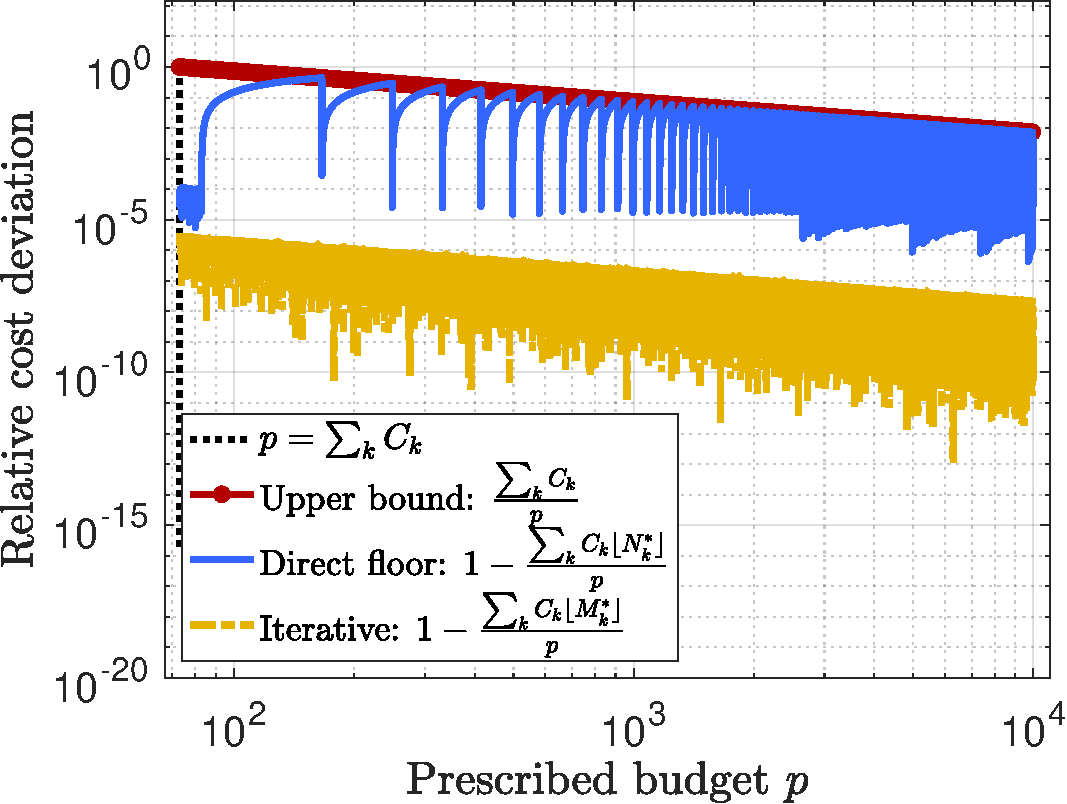
\includegraphics[width=0.48\linewidth]{./Figures/Eg1_Cost.pdf} &
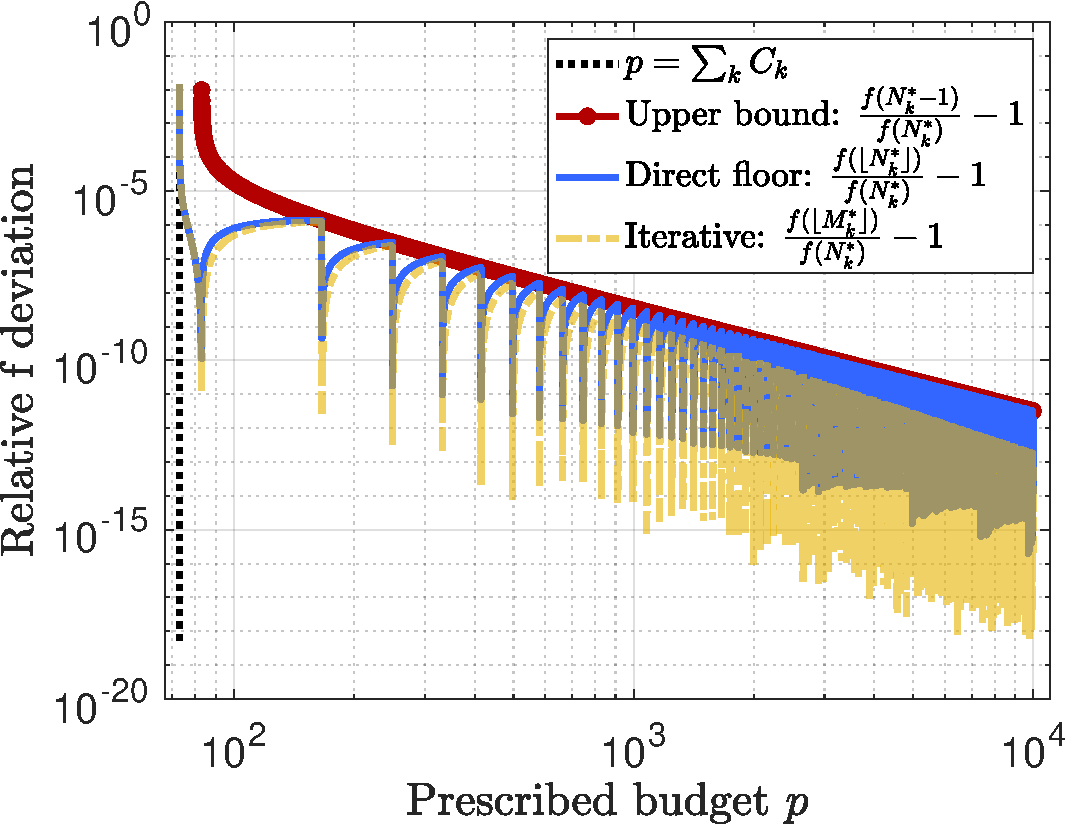
\includegraphics[width=0.48\linewidth]{./Figures/Eg1_f.pdf}
\end{tabular}
\caption{
Budget sensitivity analysis for the plasma physics example. Left: Relative cost deviation $(p - \sum_k C_k \lfloor \cdot \rfloor)/p$ versus prescribed budget $p$. Right: Relative variance deviation $(f(\lfloor \cdot \rfloor) - f(N_k^*))/f(N_k^*)$ versus prescribed budget $p$. 
} 
\label{fig:Eg1} 
\end{figure}
%

Figure~\ref{fig:Eg1} examines the sensitivity of cost utilization and variance performance to the prescribed budget $p \in [\sum_k C_k, 10^4]$, illustrating the relative performance of integer allocation schemes compared to the continuous optimum.

The left panel quantifies the budget under-utilization through the metric $p - \sum_k C_k \lfloor \cdot \rfloor$. The iterative scheme demonstrates near-perfect budget adherence across all budget levels, with deviations remaining at numerical precision levels. In contrast, direct flooring exhibits approximately six orders of magnitude greater under-utilization across most budget values. This substantial gap underscores the iterative method's ability to fully leverage available computational resources.



The variance deviation (right panel) uses the metric $\sum_k (\Delta_k/\lfloor \cdot \rfloor - \Delta_k/N_k^*)$ to measure variance inflation relative to the continuous optimum. Both integer schemes exhibit the expected variance penalty, but the iterative method consistently outperforms direct flooring across the entire budget range. Notably, the iterative scheme approaches but never exceeds the theoretical upper bound (in red) derived from the worst-case sample reduction $\sum_k (\Delta_k/(N_k^*-1) - \Delta_k/N_k^*)$, validating the theoretical guarantees established in \eqref{eq:bounds_for_floor}. The convergence of all curves (ignore sawtooth behavior) reflects the diminishing effect of integer constraints when sample sizes become substantial ($p > 10^5$).


The distinctive sawtooth patterns evident in both plots arise from the discrete nature of integer allocations. As budget $p$ increases continuously, the real-valued optimal allocation $N_k^*$ increases smoothly. However, the integer-valued allocations $\lfloor N_k^* \rfloor$ and $\lfloor M_k^* \rfloor$ remain constant until specific threshold budgets trigger discrete increments in sample counts. This creates a characteristic pattern where cost deviation increases linearly during constant-allocation intervals, followed by abrupt decreases when additional samples become affordable. Similarly, the variance deviation exhibits inverse behavior: it grows as fixed sample sizes become increasingly inadequate for larger budgets, then drops sharply when sample counts increase at threshold points.


These results collectively demonstrate that the proposed iterative method achieves superior resource utilization while minimizing statistical efficiency penalty due to integer constraints, particularly in the practically relevant budget regime where computational resources are limited.



\subsection{Second example}
We now examine a four-fidelity configuration derived from the benchmark parameters in \cite{PeWiGu:2016}, as detailed in Table~\ref{Tab:Eg2_Parameters}. This test case presents a challenging allocation scenario characterized by near-perfect inter-fidelity correlations ($\rho_{1,k} \approx 1$) and computational costs spanning five orders of magnitude. 

For a moderate budget of $p=200$, the real-valued allocation achieves an optimal variance of $f=5.0571\times10^{-5}$. Direct flooring results in substantial budget underutilization ($p \approx 179.34$) and a 15\% variance increase to $f=5.8074\times10^{-5}$, whereas the iterative scheme maintains exact budget adherence while reducing the variance penalty to just 6\% above the continuous optimum ($f=5.3495\times10^{-5}$). 

Under the more constrained budget $p=46$, direct flooring produces a degenerate estimator with infinite variance due to exclusion of the high fidelity model. The modified rounding approach restores estimator feasibility with $f=5.1658\times10^{-3}$, while the iterative method achieves a further 7\% variance reduction to $f=4.8046\times10^{-3}$ through more balanced resource distribution. Figure~\ref{fig:Eg2} demonstrates that these performance advantages persist across the entire budget spectrum, with the iterative scheme maintaining near-perfect cost utilization and consistently superior variance characteristics compared to direct flooring. The observed sawtooth patterns, arising from the discrete threshold behavior of integer allocations, further validate the theoretical framework established in equation~\eqref{eq:bounds_for_floor}. These results collectively confirm the robustness of the proposed iterative approach in handling challenging multi-fidelity configurations with extreme parameter variations. 


%
\begin{table}[ht]
\centering
\scalebox{1}{
\begin{tabular}{|c|c|c|c|c|c|c|}
\hline
Model index &1 &2 &3 &4 \\
\hline
Correlation coeff $\rho_{1,k}$ &1     &9.9999e-01  &9.9997e-01 &9.9583e-01\\
% \hline
% Standard deviation $\sigma_k$ &0.03\\
\hline
Cost &44.395 &6.8409e-01 &2.9937e-01 &1.9908e-04\\
\hline
\end{tabular}
}
\caption{Parameters from Peherstorfer's paper \cite{PeWiGu:2016}.}
\label{Tab:Eg2_Parameters}
\end{table}
%

\begin{table}[ht]
\centering
\scalebox{0.73}{
\begin{tabular}{|c|p{4.8cm}|c|c|p{4.8cm}|c|c|}
\hline
\multirow{2}{*}{Method} 
& \multicolumn{3}{c|}{$p = 46$} 
& \multicolumn{3}{c|}{$p = 200$} \\
\cline{2-7}
& Sample size & Total cost & $f$ 
& Sample size & Total cost & $f$ \\
\hline
Real-valued 
& [3.3349e-01, 2.9158e+00, 7.6071e+01, 3.2282e+04] 
& 4.6000e+01 & 2.1987e-04 
& [1.4499e+00, 1.2677e+01, 3.3074e+02, 1.4036e+05] 
& 2.0000e+02 & 5.0571e-05 \\
\hline
Integer, floor 
& [0, 2, 76, 3.2282e+04] 
& 3.0547e+01 & $\infty$ 
& [1, 12, 330, 1.4036e+05] 
& 1.7934e+02 & 5.8074e-05 \\
\hline
Modified 
& [1, 1, 2, 1.0180e+03] 
& 4.5880e+01 & 5.1658e-03 
& \multicolumn{3}{c|}{---} \\
\hline
Integer, iterative 
& [1, 1, 2, 1.6180e+03] 
& 4.6000e+01 & 4.8046e-03 
& [1, 14, 380, 1.6208e+05] 
& 2.0000e+02 & 5.3495e-05 \\
\hline
\end{tabular}
}
\caption{Comparison of real-valued and integer-valued MFMC sample allocations for small and large budgets ($p=46$ and $p=200$). The iterative integer-valued scheme achieves better cost utilization than the direct flooring approach while preserving the structure of the continuous optimizer.}
\label{tab:MFMC_integer_comparison_Eg2}
\end{table}



%
\begin{figure}[!t]\centering
\begin{tabular}{cc}
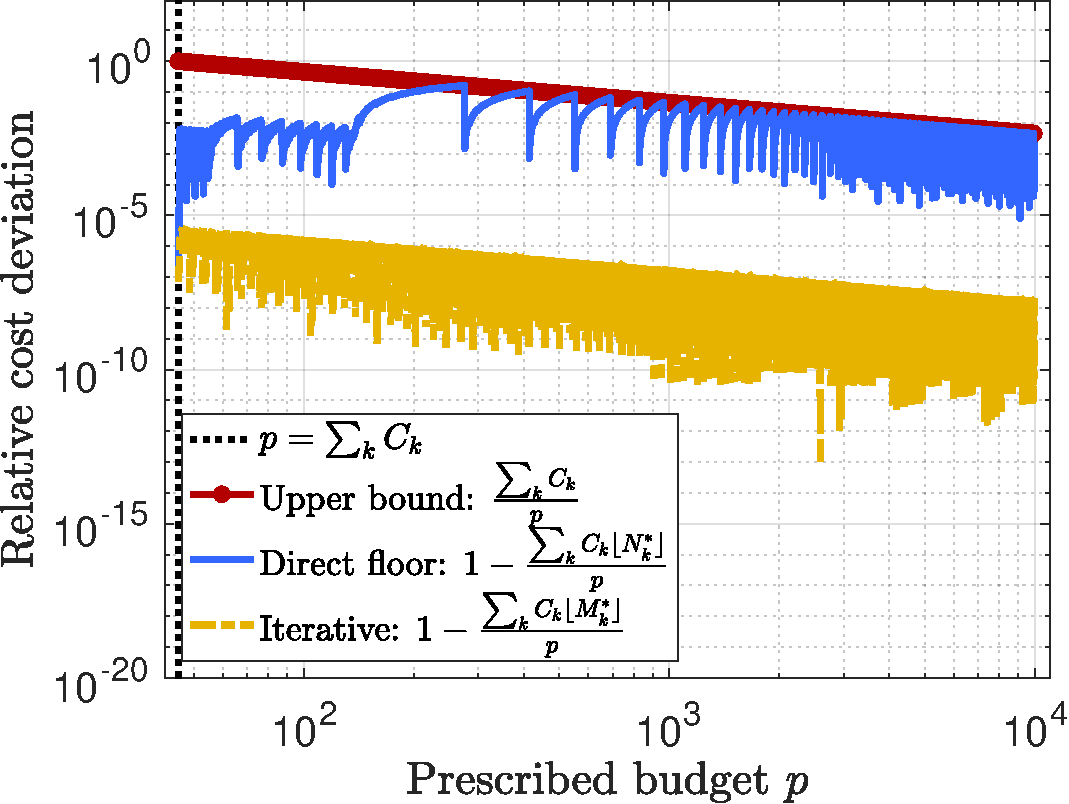
\includegraphics[width=0.48\linewidth]{./Figures/Eg2_Cost.pdf} &
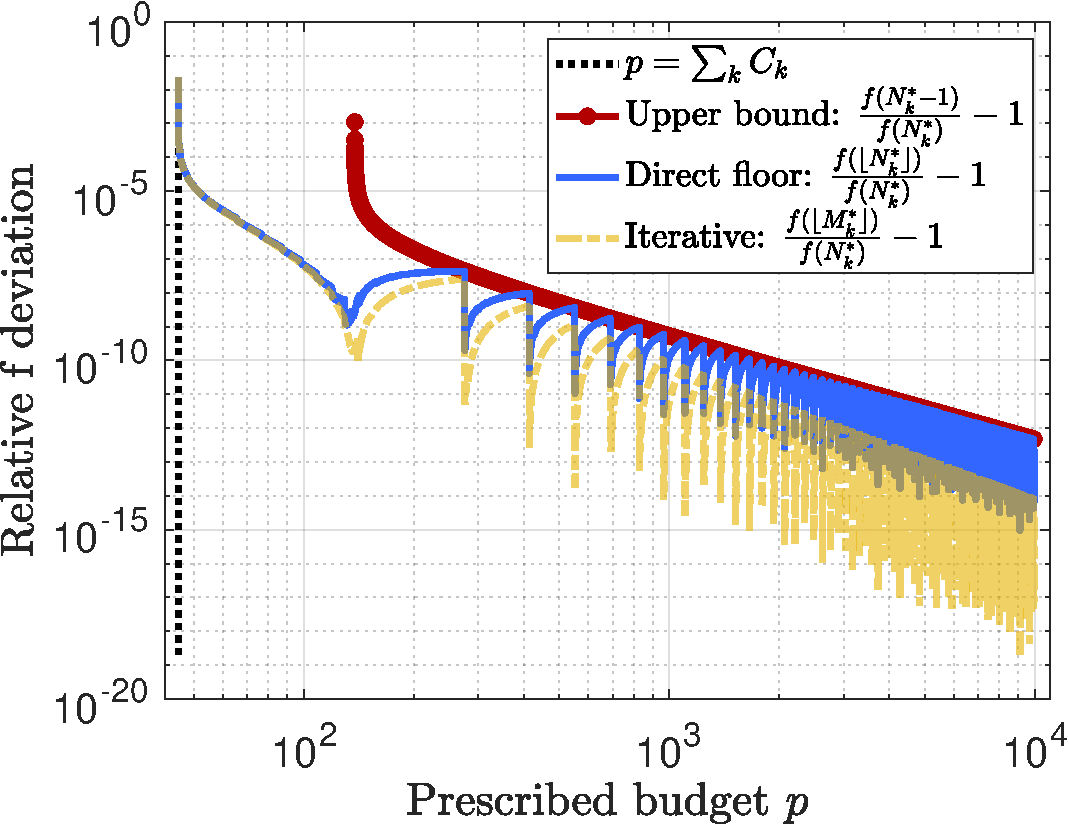
\includegraphics[width=0.48\linewidth]{./Figures/Eg2_f.pdf}
\end{tabular}
\caption{
Left: Relative cost deviation $(p - \sum_k C_k \lfloor \cdot \rfloor)/p$ versus prescribed budget $p$. Right: Relative variance deviation $(f(\lfloor \cdot \rfloor) - f(N_k^*))/f(N_k^*)$ versus prescribed budget $p$.
} 
\label{fig:Eg2} 
\end{figure}
%












% %
% \begin{table}[ht]
% \centering
% \scalebox{0.6}{
% \begin{tabular}{|c|c|c|c|c|c|c|c|c|c|}
% \hline
% Total cost $P$ &73.05 &73.051 &73.052 &73.053 &73.054 &73.055 &73.056\\
% \hline
% Sample size (real valued) &[1,   134,   588   2540,  21100] &[1,   135,   588,   2541,  21101]&same &same &[1,   135,   588,   2541,  21102] &same &same\\
% \hline
% Sample size (integer program) &[1, 2, 3, 11, 97]&[1, 2, 3, 12, 99]&-&-&-&-&-\\
% \hline
% CPU time for integer program [s] & 0.27 &0.32 &$>$ 1000 &$>$ 1000 &$>$ 1000 &$>$ 1000 &$>$ 1000\\
% \hline
% \end{tabular}
% }
% \caption{Sample size for real-valued optimization and integer optimization.}
% \label{Tab:Sample_Size}
% \end{table}
% %








% %
% \begin{table}[ht]
% \centering
% \scalebox{1}{
% \begin{tabular}{|c|c|c|c|c|c|c|c|c|c|}
% \hline
% &Sample size &Total cost $p$ &$f$\\
% \hline
% Real valued &[2.4129e+00 3.6959e+02 1.6102e+03 6.9567e+03 5.7770e+04]&200&2.1645e-04\\
% \hline
% Integer, floor &[2, 369, 1610, 6956, 57769]&1.698561e+02&2.5580e-04\\
% \hline
% Integer, iterative&[2, 836, 3644, 15744, 130749]&1.999999e+02&2.4138e-04\\
% % \hline
% % CPU time for integer program [s] & 0.27\\
% \hline
% \end{tabular}
% }
% \caption{Sample size for real-valued optimization and integer optimization for $p=200$.}
% \label{Tab:Eg1_p_large}
% \end{table}
% %

% %
% \begin{table}[ht]
% \centering
% \scalebox{1}{
% \begin{tabular}{|c|c|c|c|c|c|c|c|c|c|}
% \hline
% &Sample size &Total cost $p$ &$f$\\
% \hline
% Real valued &[8.8106e-01,   1.3495e+02,   5.8795e+02,   2.5402e+03,  2.1095e+04]&73.03&5.9275e-04\\
% \hline
% Integer, floor &[0,         134,         587,        2540,  21094]&8.7045&$\infty$\\
% \hline
% Modified &[1,     1,     1,     7,    62]&7.302859e+01&2.4834e-02\\
% % \hline
% \hline
% Integer, iterative &[1,     1,     1,     7,    67]&7.302993e+01&2.3668e-02\\
% % \hline
% % CPU time for integer program [s] & 0.27\\
% \hline
% \end{tabular}
% }
% \caption{Sample size for real-valued optimization and integer optimization for $p=73.03$.}
% \label{Tab:Eg1_p_small}
% \end{table}
% %



% %
% \begin{table}[ht]
% \centering
% \scalebox{1}{
% \begin{tabular}{|c|c|c|c|c|c|c|c|c|c|}
% \hline
% &Sample size &Total cost $p$ &$f$\\
% \hline
% Real valued &[1.449950e+00 1.267731e+01 3.307436e+02 1.403572e+05]&200&5.0571e-05\\
% \hline
% Integer, floor &[1, 12, 330, 140357]&1.793385e+02&5.8074e-05\\
% \hline
% Integer, iterative&[1, 14, 380, 162081]&1.999999e+02&5.3495e-05\\
% % \hline
% % CPU time for integer program [s] & 0.27\\
% \hline
% \end{tabular}
% }
% \caption{Sample size for real-valued optimization and integer optimization for $p=200$.}
% \label{Tab:Eg2_p_large}
% \end{table}
% %



% %
% \begin{table}[ht]
% \centering
% \scalebox{1}{
% \begin{tabular}{|c|c|c|c|c|c|c|c|c|c|}
% \hline
% &Sample size &Total cost $p$ &$f$\\
% \hline
% Real valued &[3.334886e-01 2.915781e+00 7.607103e+01 3.228216e+04]&46&2.1987267e-04\\
% \hline
% Integer, floor &[0, 2, 76, 32282]&3.054700e+01&$\infty$\\
% \hline
% Modified &[1, 1, 2, 1018]&4.588049e+01&5.1658e-03\\
% % \hline
% \hline
% Integer, iterative &[1, 1, 2, 1618]&4.599994e+01&4.8046e-03\\
% % \hline
% % CPU time for integer program [s] & 0.27\\
% \hline
% \end{tabular}
% }
% \caption{Sample size for real-valued optimization and integer optimization for $p=46$.}
% \label{Tab:Eg2_p_small}
% \end{table}
% %